\documentclass[aspectratio=169]{beamer}

\usepackage[spanish]{babel}
\usepackage[utf8]{inputenc}
\usepackage[T1]{fontenc}
\usepackage{graphicx}
\usepackage{booktabs}
\usepackage{tikz}
\usetikzlibrary{positioning}

\usetheme{Madrid}
\usecolortheme{default}
\setbeamertemplate{navigation symbols}{}

\title{Sistema de vision artificial para un sumobot}
\subtitle{Seguimiento de carril y expulsion de objetos}
\author{Juan Jose Prado Neira}
\date{Junio de 2026}

\begin{document}

\begin{frame}
  \titlepage
\end{frame}

\begin{frame}{Objetivo}
  \begin{itemize}
    \item Controlar un sumobot usando una ESP32-CAM y procesado en portatil.
    \item Navegar entre dos lineas del carril.
    \item Detectar objetos en la trayectoria y apartarlos fuera del carril.
    \item Mantener control manual y parada segura durante las pruebas.
  \end{itemize}
\end{frame}

\begin{frame}{Arquitectura general}
  \centering
  \begin{tikzpicture}[node distance=1.4cm, every node/.style={draw, rounded corners, align=center, minimum width=2.3cm, minimum height=0.8cm}]
    \node (cam) {ESP32-CAM\\video UDP};
    \node[right=of cam] (pc) {Portatil\\OpenCV};
    \node[right=of pc] (dec) {Decision\\auto/manual};
    \node[right=of dec] (bot) {ESP32 motores\\comandos UDP};
    \draw[->, thick] (cam) -- (pc);
    \draw[->, thick] (pc) -- (dec);
    \draw[->, thick] (dec) -- (bot);
  \end{tikzpicture}
\end{frame}

\begin{frame}{Recepcion y visualizacion}
  \begin{itemize}
    \item La ESP32-CAM envia JPEG fragmentado por UDP.
    \item El receptor reconstruye frames y conserva el ultimo frame valido ante perdidas cortas.
    \item La ventana de OpenCV muestra camara, mascara, ROI y vista de depuracion.
  \end{itemize}
\end{frame}

\begin{frame}{Procesado de imagen}
  \begin{itemize}
    \item ROI inferior y transformacion de perspectiva configurable.
    \item Mascara de lineas oscuras por contraste local, umbral absoluto y morfologia.
    \item Estimacion del centro del carril con una o dos lineas visibles.
    \item Salida: accion sugerida, confianza, offset y razon de deteccion.
  \end{itemize}
\end{frame}

\begin{frame}{Deteccion de objetos}
  \begin{itemize}
    \item Segmentacion de regiones oscuras de baja saturacion.
    \item Filtros por area, relleno, aspecto y contacto con bordes.
    \item Fusion de objetos apilados para tratar un obstaculo como una sola entidad.
    \item Exclusion del objeto en la mascara de linea para evitar falsos carriles.
  \end{itemize}
\end{frame}

\begin{frame}{Control y protocolo de expulsion}
  \begin{enumerate}
    \item Enfocar el objeto hasta centrarlo.
    \item Aproximarse durante un numero fijo de frames.
    \item Empujar con curva lateral.
    \item Reincorporarse marcha atras con la curva configurada.
  \end{enumerate}
\end{frame}

\begin{frame}{Interfaz de uso}
  \begin{itemize}
    \item \texttt{Enter}/espacio: activar o bloquear movimiento.
    \item \texttt{m}: alternar automatico y manual.
    \item Manual: \texttt{w}, \texttt{a}, \texttt{d}, \texttt{s}.
    \item Automatico con override: \texttt{f}, \texttt{l}, \texttt{r}, \texttt{s}.
    \item \texttt{q}/Esc: salir enviando parada al robot.
  \end{itemize}
\end{frame}

\begin{frame}{Resultados registrados}
  \begin{table}
    \centering
    \begin{tabular}{lrrr}
      \toprule
      Sesion & Frames & Tiempo (s) & FPS \\
      \midrule
      13:04 & 1.518 & 54,74 & 27,73 \\
      13:04b & 2.407 & 87,06 & 27,65 \\
      13:06 & 2.993 & 107,50 & 27,84 \\
      13:08 & 11.973 & 428,40 & 27,95 \\
      \midrule
      Total & 18.891 & 677,70 & 27,88 \\
      \bottomrule
    \end{tabular}
  \end{table}
\end{frame}

\begin{frame}{Ejemplo de ejecucion}
  \centering
  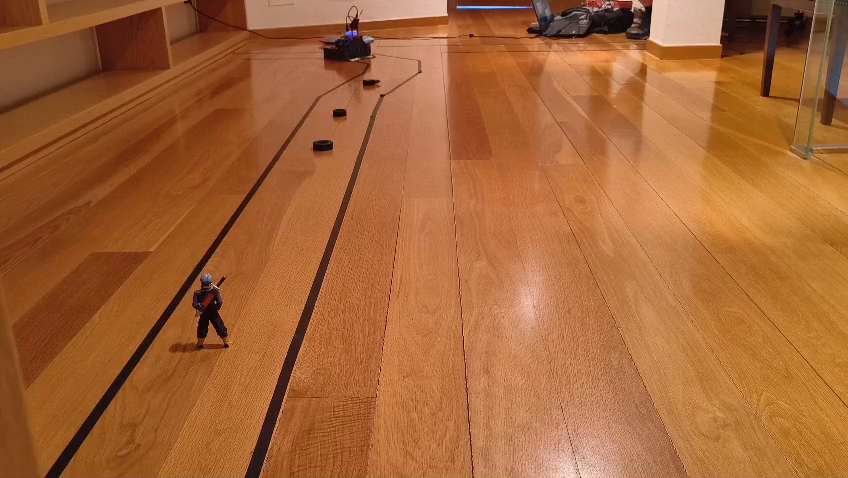
\includegraphics[width=0.92\linewidth]{../paper/figures/demo_frame.png}
\end{frame}

\begin{frame}{Conclusiones}
  \begin{itemize}
    \item Integracion funcional de video UDP, OpenCV, decision y control del robot.
    \item Arquitectura por bloques facil de ajustar mediante JSON.
    \item Resultados estables en laboratorio: alrededor de 28 FPS registrados.
    \item Mejoras futuras: odometria, medicion de latencia y segmentacion aprendida.
  \end{itemize}
\end{frame}

\end{document}
